
\documentclass{hcmutarticle}

% gói để tạo chữ giả, xóa đi khi viết báo cáo
\usepackage{lipsum}
\usepackage{listings}
\usepackage{color}

\definecolor{dkgreen}{rgb}{0,0.6,0}
\definecolor{gray}{rgb}{0.5,0.5,0.5}
\definecolor{mauve}{rgb}{0.58,0,0.82}

\lstset{frame=tb,
  language=Java,
  aboveskip=3mm,
  belowskip=3mm,
  showstringspaces=false,
  columns=flexible,
  basicstyle={\small\ttfamily},
  numbers=none,
  numberstyle=\tiny\color{gray},
  keywordstyle=\color{blue},
  commentstyle=\color{dkgreen},
  stringstyle=\color{mauve},
  breaklines=true,
  breakatwhitespace=true,
  tabsize=3
}

% create the header for this file
\fancyhead[RO, LE]{\bf Tìm hiểu về Apache Kafka, Apache Storm}


\begin{document}
\thispagestyle{empty}
\begin{center}
\LARGE\bfseries IKORN SOLUTIONS \\
\end{center}

\begin{center}

\includegraphics[scale=1]{ikorn.jpg}\\[1cm]
\end{center}

\vspace{1cm}

\begin{center}
\Large \bfseries DOCUMENT FOR IFP PROJECT\\[0.5cm]
\end{center}
\rule{\textwidth}{1pt}
\vspace{2pt}
\begin{center}
\Huge
\begin{tabular}{@{}l}
Tìm hiểu về Apache kafka và Apache Storm\\[6pt]
\end{tabular}
\end{center}
\rule{\textwidth}{1pt}\\[1cm]

\vspace{2cm}

\begin{minipage}[t]{0.60\linewidth}
\textbf{}:
\end{minipage}
\begin{minipage}[t]{0.40\linewidth}
\textbf{Người thực hiện:}\\
Nguyễn Quốc Long
\end{minipage}

\vspace{3cm}

\begin{center}

\textbf{TP.Hồ Chí Minh},
25/07/2018.

\end{center}



\newpage

\tableofcontents 

\newpage

\title{Tìm hiểu về Apache Kafka và Apache storm}

\author{  Nguyễn Quốc Long\inst{1}} 



\maketitle



\begin{abstract}
Tài liệu tìm hiểu về Apache Kafka và Apache Storm


\end{abstract}

\begin{keywords}
algorithm, apache storm, apache kafaka, big data  ...
\end{keywords} 


\section{Giới thiệu}

\textbf{Apache kafka} 
là hệ thống truyền tin nhắn được xây dựng cho big data. Kafka
cho phép ứng dụng xây dựng trên các nền tảng khác nhau và giao
tiếp với nhau thông qua việc truyền thông điệp theo cơ chế bất
đồng bộ.

\textbf{Apache storm}
là hệ thống để xử lý streaming data trong thời gian thực. Apache
Storm hỗ trợ nhiều ngôn ngữ như: scala, python, Javascript,
java, vv...

\newpage

%%%%%%%%%%%%%%
\section{Tóm tắt nội dung}\label{survey}
Bài tìm hiểu này sẽ trình bày cá nội dung sau đây: \\
$-$ Khái niệm cơ bản về apache Kafka\\
$-$ Khái niệm cơ bản về apache Storm\\
$-$ Apache Kafka  phối hợp với Apache storm\\
%{\bfseries Sau đây là cách trích dẫn tài liệu tham khảo theo
%quy định của Bộ Giáo Dục và Đào Tạo:}\\
%%%%%%%%%%%%%%
\section{Nội dung tìm hiểu}\label{dev}

\subsection{Apache kafka}

Apache kafka là hệ thống truyền tải thông điệp được xây dựng
trên hệ thống có thể mở rộng dễ dàng cho big data. \\
Kafka khác so với các hệ thống truyền tin truyền thống ở những
điểm sau: \\
$-$ Được thiết kế để scale horizontally, bằng cách thêm vào
nhiều hơn các server thông thường\\
$-$ Cung cấp khả năng throughput cao cho cả producer and
customer\\
$-$ Hỗ trợ cả bath và real-time use case\\
$-$ Không hỗ trợ JMS (Java mesage Service Concepts), Java's
mesage-oriented middleware API.

\begin{center}
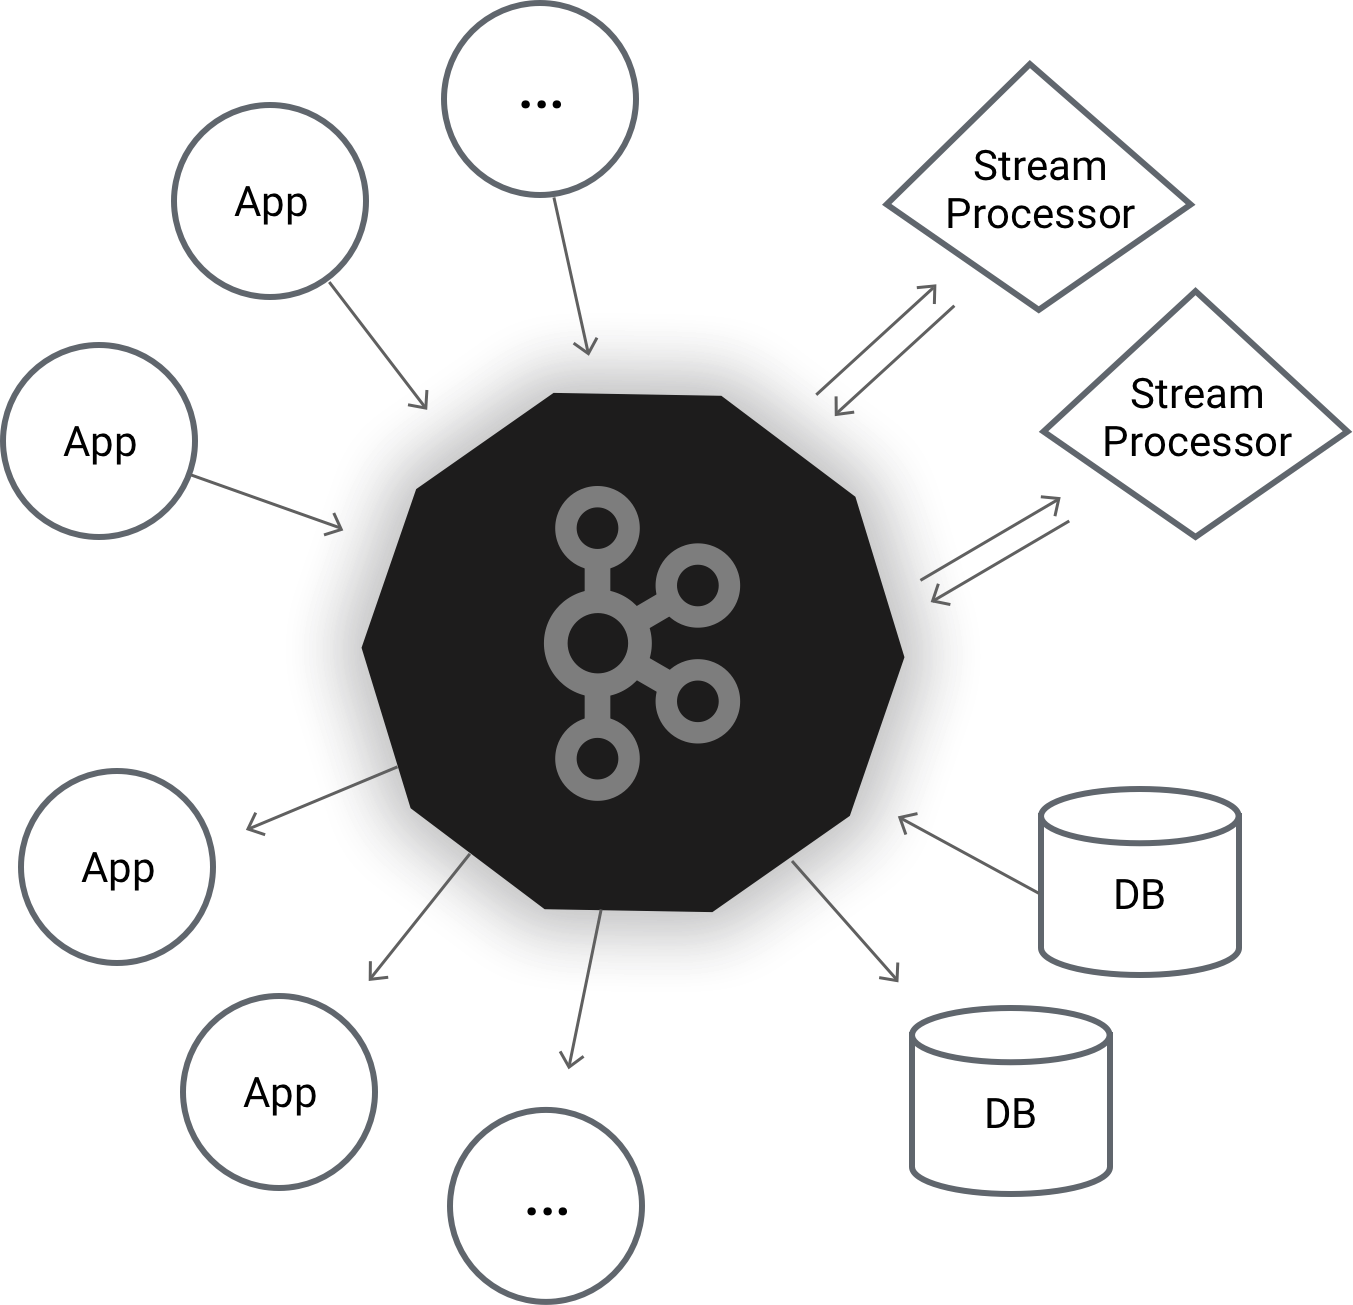
\includegraphics[scale=0.2]{image/kafka_diagram.png}\\[1cm]
\end{center}

\subsubsection{kafka's architecture}.\\
Trước khi ta tìm hiểu kiến trúc của kafka, ta cần biết các thuật
ngữ (terminology) sau đây:
\begin{itemize}
\item A producer là process có thể publish a message to topic
\item A consumer is a process that can subscribe to one or more
topics and consume messages published to topics.
\item A topic category is the name of the feed to which messages
are published.
\item A broker is the process running on single machine.
\item A cluster is a group of brokers working together.
\end{itemize}

\begin{center}
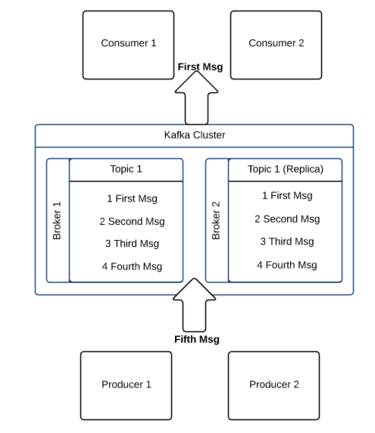
\includegraphics[scale=0.8]{image/kafka-architecture.png}\\[1cm]Figure 1. Architecture of a Kafka message system.
\end{center}

Kafka's architecture is very simple, which can result in better
performance and throughput in some systems.\\
Every topic in Kafka is like a simple log file. When a producer
publishes a message, the Kafka server appends it to the end of
the log file for its given topic.

The Server also assigns an offset, which is a number used to
permanently identify each message. As the number of messages
grows, the value of each offset increases; for example if the
producer publishes three message the first one might get an
offset of 1, the second an offset of 2, and the thrid an offset
of 3.

When the Kafka consumer first starts, it will send a pull
request to the server, asking to retrieve any messanges for a
particular topic with an offset value higher than 0. The server
will check the log file for that topic and return three new
massages. The consumer will process the messages, then send a
request for messages with an offset higher than 3, so on.



In Kafka, the client is reponsible for remmberiing the the
offset count aand retieving message. The Kafka server doesn't
track or manage message consumption. By default, a Kafka server
will keep message for seven days. A backgroud thread in the
server checks and deletes messages that are seven day or older.
A consumer can access messages as long as they are on the
server. It can read a message multiple times, and even read
messages in reverse order od receipt. But if the consumer fails
to retrieve the message before the seven days are up, it will
miss that message.
\subsubsection{Quick setup and demo}

We'll build a custom application in this tutorial, but let's
start by installing and testing a Kafka instance with an
out-of-the-box producer and consumer.\\
\begin{enumerate}
\item Visit the Kafka download page to install the most recent
version.
  \item Extract the binaries into a software/kafka folder.
\item Change your current directory to point to the new folder.\item Start the Zookeeper server by executing the command:
bin/zookeeper-server-start.sh config/zookeeper.properties.
\item Start the Kafka server by executing:
bin/kafka-server-start.sh config/server.properties.
\item Create a test topic that you can use for testing:
bin/kafka-topics.sh --create --zookeeper localhost:2181
--replication-factor 1 --partitions 1 --topic javaworld.
\item Start a simple console consumer that can consume messages
published to a given topic, such as javaworld:
bin/kafka-console-consumer.sh --zookeeper localhost:2181 --topic
javaworld --from-beginning.
\item Start up a simple producer console that can publish
messages to the test topic: bin/kafka-console-producer.sh
--broker-list localhost:9092 --topic javaworld.
\item Try typing one or two messages into the producer console.
Your messages should show in the consumer console.
\end{enumerate}
\subsection{Apache Storm}
\subsubsection{What is Apache Storm ?\\}
\textbf{Apache Storm} is a distributed real-time computation
system for processing large volumes of high-velocity data.\\
Apache storm is extremely fast, with the ability to process over
a million records per second per node on a cluster of modest
size.\\
Enterprises harness this speed and combine it with other data
access applications in Hadoop to prevent undesirable events or
to optimize positive outcomes.\\
\subsubsection{Feature of Apache Storm}
\begin{enumerate}
\item Storm is simple and developers can write Storm topologies
using any programming language.
\item A Storm topology consists of “Spouts” and “Bolts”.
\item The “data” in a Storm topology is called a “Tuple”.
\end{enumerate}

\subsubsection{Characteristic of Apache Storm\\}
Five characteristics make Storm ideal for real-time data
processing workloads is :
\begin{enumerate}
\item \textbf{Fast} – benchmarked as processing one million 100
byte messages per second per node
\item \textbf{Scalable} – with parallel calculations that run
across a cluster of machines
\item \textbf{Fault-tolerant} – when workers die, Storm will
automatically restart them. If a node dies, the worker will be
restarted on another node.
\item \textbf{Reliable} – Storm guarantees that each unit of
data (tuple) will be processed at least once or exactly once.
Messages are only replayed when there are failures.
\item \textbf{Easy to operate} – standard configurations are
suitable for production on day one. Once deployed, Storm is easy
to operate
\end{enumerate}
\subsubsection{Quick setup and demo\\}
\textbf{In sumary, the steps are:}
\begin{itemize}
\item Download a Storm release, unpack it, and put the unpacked
bin/ directory on your PATH.
\item To be able to start and stop topologies on a remote
cluster, put the cluster information in ~/.storm/storm.yaml.
\item A Storm development environment has everything installed
so that you can develop and test Storm topologies in local mode,
package topologies for execution on a remote cluster, and
submit/kill topologies on a remote cluster.
\end{itemize}

\subsubsection{Abstractions in Storm: spouts, bolts, and
topologies\\}
There are just three abstractions in Storm: spouts, bolts, and
topologies.
\begin{enumerate}
\item \textbf{A spout} is a source of streams in a computation.
Typically a spout reads from a queueing broker such as Kestrel,
RabbitMQ, or Kafka, but a spout can also generate its own stream
or read from somewhere like the Twitter streaming API. Spout
implementations already exist for most queueing systems.
\item \textbf{A bolt} processes any number of input streams and
produces any number of new output streams. Most of the logic of
a computation goes into bolts, such as functions, filters,
streaming joins, streaming aggregations, talking to databases,
and so on.
\item \textbf{A topology} is a network of spouts and bolts, with
each edge in the network representing a bolt subscribing to the
output stream of some other spout or bolt. A topology is an
arbitrarily complex multi-stage stream computation. Topologies
run indefinitely when deployed.
\end{enumerate}
\begin{center}
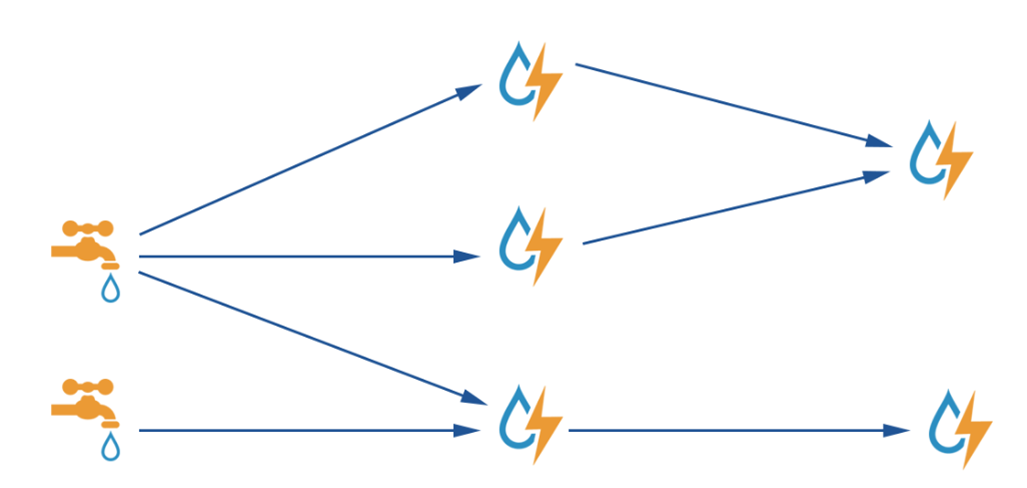
\includegraphics[scale=0.6]{image/abstract-storm.png}\\[0.5cm]
Figure 2. Three abstractions in Storm: spouts, bolts, and
topologies..
\end{center}
%%%%%%%%%%%%%%%%%%%%%%%%%%%%%%%%
\subsubsection{Core Storm Concepts}.\\
Developing a Storm application requires an understanding of the
following basic concepts.\\
Table 4.1. Storm Concepts

\begin{center}
\begin{tabular} {| l | p{10cm} |}
	\hline
		\textbf{Storm Concept} & \textbf{Descripition}\\
	\hline
		Tuple & A named list of values of any data type. A Tuple is the
native data structure used by storm.\\
	\hline
		Stream & An bounded sequence of tuples.\\
	\hline
		Spout & Generates a stream from a realtime data source.\\
	\hline
		Bolt & Contains data processing, persistence, and messaging
alert logic.
		Can also emit tuples for downstream bolts.\\
	\hline
	Topology & A group of spouts and bolts wired together into a
wordflow.
	A Storm application.\\
	\hline
	Processing Reliability & Storm guarantee about the delivery of
tuples in a topology.\\
	\hline
	Workers & A storm process. A worker may run one oe more
executors.\\
	\hline
	Executor & A storm thread launched by Storm worker.
A executor may run one or more task.\\
	\hline
		Tasks & A Storm job from a spout or bolt.\\
\hline
Parallelism & Attribute of distributed data oricessing that determines how many jobs are processed simultaneously for a topology.
Topology developers adjust parallelism to tune their applications.\\
\hline
Process Controller & Monotors and restarts failed storm processes. Examples include supervisord, monit, and daemontools.\\
\hline
Master/Numbus Node & The host isn a multi-node Storm cluster that runs a process controller (such as supervisord) and the Storm numbus, ui, and other related daemons. The process controller is responsible for restarting failed process controller deamons on slave node. The Nimbus node is a thrift service that is responsible for distributing code around the cluster, addigning tasks to machines, and monitoring for failures.\\
\hline
Slave Node & A host in a multi-node Storm cluster that runs a process controller daemon, such as supervisor, as well as the worker processes that run Storm topologies. The process controller daemon is responsible for restaring failed worker processes.\\
\hline
\end{tabular}
\end{center}




%With width specified:
%\begin{center}
%    \begin{tabular}{ | l | l | l | p{5cm} |}
%    \hline
%    Day & Min Temp & Max Temp & Summary \\ \hline
%    Monday & 11C & 22C & A clear day with lots of sunshine.  
%However, the strong breeze will bring down the temperatures. \\
%\hline
%Tuesday & 9C & 19C & Cloudy with rain, across many northern
%regions. Clear spells
%    across most of Scotland and Northern Ireland, 
%    but rain reaching the far northwest. \\ \hline
%Wednesday & 10C & 21C & Rain will still linger for the morning. Conditions will improve by early afternoon and continue 
%    throughout the evening. \\
%    \hline
%    \end{tabular}
%\end{center}

\subsubsection{Spouts\\}
All spouts must implement the org.apache.storm.topology.IRichSpout interface
from the core-storm API. BaseRichSpout is the most basic implementation, but there are
several others, including ClojureSpout, DRPCSpout, and FeederSpout. In addition,
Hortonworks provides a Kafka spout to ingest data from a Kafka cluster. The following
example, RandomSentenceSpout, is included with the storm-starter connector
installed with Storm at /usr/lib/storm/contrib/storm-starter.

\begin{lstlisting}
package storm.starter.spout;
        import org.apache.storm.spout.SpoutOutputCollector;
        import org.apache.storm.task.TopologyContext;
        import org.apache.storm.topology.OutputFieldsDeclarer;
        import org.apache.storm.topology.base.BaseRichSpout;
        import org.apache.storm.tuple.Fields;
        import org.apache.storm.tuple.Values;
        import org.apache.storm.utils.Utils;
        import java.util.Map;
        import java.util.Random;

public class RandomSentenceSpout extends BaseRichSpout {
    SpoutOutputCollector _collector;
    Random _rand;

    @Override
    public void open(Map conf, TopologyContext context, SpoutOutputCollector
            collector) {
        _collector = collector;
        _rand = new Random();
    }

    @Override
    public void nextTuple() {
        Utils.sleep(100);
        String[] sentences = new String[]{"the cow jumped over the moon", "an
                apple a day keeps the doctor away", " four score and seven years ago", " snow
                white and the seven dwarfs", " i am at two with nature" };
                String sentence = sentences[_rand.nextInt(sentences.length)];
        _collector.emit(new Values(sentence));
        }
        @Override
        public void ack (Object id){
        }
        @Override
        public void fail (Object id){
        }
        @Override
        public void declareOutputFields (OutputFieldsDeclarer declarer){
            declarer.declare(new Fields("word"));
        }
    }
\end{lstlisting}
%%%%%%%%%%%%%%%%%%%%
\subsubsection{Bolts\\}
All bolts must implement the IRichBolt interface. BaseRichBolt is the most
basic implementation, but there are several others, including BatchBoltExecutor,
ClojureBolt, and JoinResult. The following example, TotalRankingsBolt.java,
is included with storm-starter and installed with Storm at /usr/lib/storm/
contrib/storm-starter.
\begin{lstlisting}
package storm.starter.bolt;
import org.apache.storm.tuple.Tuple;
import org.apache.log4j.Logger;
import storm.starter.tools.Rankings;
/**
* This bolt merges incoming {@link Rankings}.
* <p/>
* It can be used to merge intermediate rankings generated by {@link
IntermediateRankingsBolt} into a final,
* consolidated ranking. To do so, configure this bolt with a globalGrouping
on {@link IntermediateRankingsBolt}.
*/
public final class TotalRankingsBolt extends AbstractRankerBolt {
private static final long serialVersionUID = -8447525895532302198L;
private static final Logger LOG = Logger.getLogger(TotalRankingsBolt.class);
public TotalRankingsBolt() {
super();
}
public TotalRankingsBolt(int topN) {
super(topN);
}
public TotalRankingsBolt(int topN, int emitFrequencyInSeconds) {
Hortonworks Data Platform December 15, 2017
17
super(topN, emitFrequencyInSeconds);
}
@Override
void updateRankingsWithTuple(Tuple tuple) {
Rankings rankingsToBeMerged = (Rankings) tuple.getValue(0);
super.getRankings().updateWith(rankingsToBeMerged);
super.getRankings().pruneZeroCounts();
}
@Override
Logger getLogger() {
return LOG;
}
}
\end{lstlisting}
%%%%%%%%%%%%%%%%%%%%
\subsubsection{Processing Reliability\\}
Storm provides two types of grarantees when processing tuples for a Storm topology.

\textbf{Table 4.3. Processing Guarantees}
\begin{center}
	\begin{tabular}{|l| p{12cm} |}
		\hline
			\textbf{Guarantee} & \textbf{Description} \\
		\hline
			At least once & Reliable; Tuples are processed at least once, but may be processes more than once. use when subsecond latency is required and for unordered idempotent operations.\\
		\hline
			Exactly once & Reliable; Tuples are processed only once.( this feature requires the use of a Trident spout and the Trident API. For more information, see Trident concepts).\\
		\hline
	\end{tabular}	
\end{center}

%%%%%%%%%%%%%%%%%%%%
\subsubsection{Stream Grouping\\}
Stream grouping allows Storm developers to control how tuples are routed to bolts in a
workflow. The following table describes the stream groupings available.

%%% Begin table
\textbf{Table 4.2. Stream Groupings}
\begin{center}
	\begin{tabular}{|l| p{12cm} |}
		\hline
		\textbf{Stream Grouping} & \textbf{Description}\\
		\hline
		Shuffle & Sends tuples to bolts in random, round robin sequence. Use for atomic operations, such as math.\\
		\hline
		Fields & Sends tuples to a bolt based on one or more fields in the
tuple. Use to segment an incoming stream and to count
tuples of a specified type.\\
		\hline
		All & Sends a single copy of each tuple to all instances of a
receiving bolt. Use to send a signal, such as clear cache or
refresh state, to all bolts.\\
		\hline
		Custom & Customized processing sequence. Use to get maximum
flexibility of topology processing based on factors such as
data types, load, and seasonality. \\
		\hline
		Direct & Source decides which bolt receives a tuple.
Global Sends tuples generated by all instances of a source to a
single target instance. Use for global counting operations.\\
		\hline
	\end{tabular}
\end{center}
%%% end table
Storm developers specify the field grouping for each bolt using methods on the
TopologyBuilder.BoltGetter inner class, as shown in the following excerpt from the
the WordCountTopology.java example included with storm-starter.
...
\begin{lstlisting}
TopologyBuilder builder = new TopologyBuilder();
builder.setSpout("spout", new RandomSentenceSpout(), 5);
builder.setBolt("split", new SplitSentence(), 8).shuffleGrouping("spout");
builder.setBolt("count", new WordCount(), 12).fieldsGrouping("split", new
Fields("word"));
\end{lstlisting}

The first bolt uses shuffle grouping to split random sentences generated with the
RandomSentenceSpout. The second bolt uses fields grouping to segment and perform a
count of individual words in the sentences.
%%%%%%%%%%%%%%%%%%
\subsubsection{Topologies\\}
\begin{center}
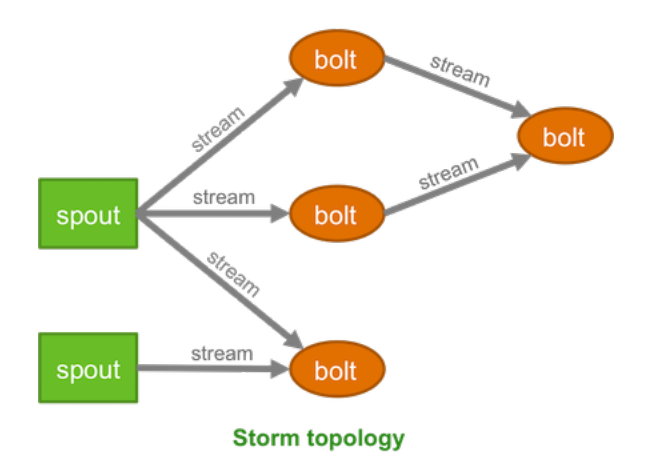
\includegraphics[scale=0.3]{image/topologyPNG.PNG}\\[0.5cm]
Figure 3. Storm Topology.
\end{center}

The TopologyBuilder class is the starting point for quickly writing Storm topologies
with the storm-core API. The class contains getter and setter methods for the spouts and
bolts that comprise the streaming data workflow, as shown in the following sample code.

\begin{lstlisting}
TopologyBuilder builder = new TopologyBuilder();
builder.setSpout("spout1", new BaseRichSpout());
builder.setSpout("spout2", new BaseRichSpout());
builder.setBolt("bolt1", new BaseBasicBolt());
builder.setBolt("bolt2", new BaseBasicBolt());
builder.setBolt("bolt3", new BaseBasicBolt());
\end{lstlisting}
%%%%%%%%%%%%%%
\subsubsection{Workers, Executors, and tasks\\}
Apache Storm processes, called workers, run on predefined ports on the machine that hosts Storm.\\
* Each worker process can run one or more executors, or threads, or threads, where each executor is a thread spawned by the worker process.\\
* Each executor runs one or more tasks from the same component, where a component is a spout or bolt from a topology.\\
Here is a simple illustration of their relationships:\\

\begin{center}
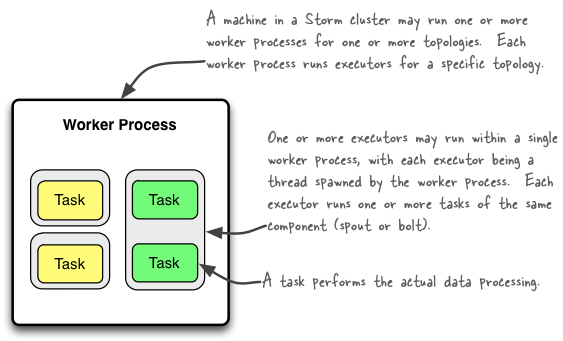
\includegraphics[scale=1.2]{image/relationships-worker-processes-executors-tasks.png}\\[0.5cm]
Figure 4. What makes a running topology: worker processes, executors and tasks.
\end{center}
%%%%%%%%%%%%%%
\subsubsection{Parallelism\\}
Distributed applications take advantage of horizontally-scaled clusters by dividing
computation tasks across nodes in a cluster. Storm offers this and additional finer-grained
ways to increase the parallelism of a Storm topology:\\
\begin{itemize}
\item Inscease the number of work
\item Increase the number of executors
\item Increase the number of task
\end{itemize}
Here is the relevant code:\\
\begin{lstlisting}
Config conf = new Config();
conf.setNumWorkers(2); 
//use two worker processes

topologyBuilder.setSpout("blue-spout", new BlueSpout(), 2); 
// set parallelism hint to 2

topologyBuilder.setBolt("green-bolt", new GreenBolt(), 2)
               .setNumTasks(4)
               .shuffleGrouping("blue-spout");

topologyBuilder.setBolt("yellow-bolt", new YellowBolt(), 6)
               .shuffleGrouping("green-bolt");

StormSubmitter.submitTopology(
        "mytopology",
        conf,
        topologyBuilder.createTopology()
    ); 
\end{lstlisting}

%%%%%%%%%%%%%%%%%%%%
\section{Apache Storm integration with Apache Kafka}

\begin{center}
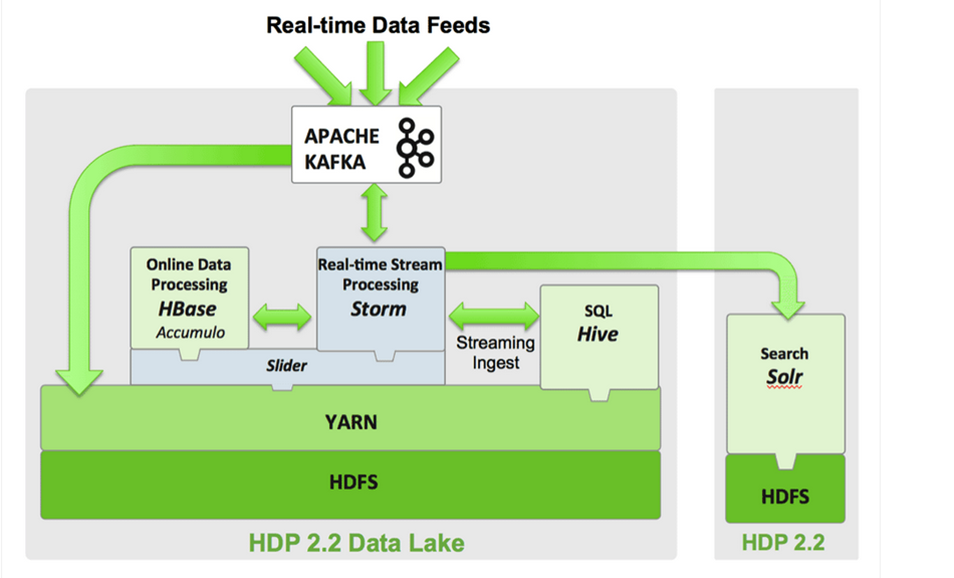
\includegraphics[scale=0.6]{image/storm-kafka-1.png}\\[0.5cm]
Figure 3. Apache Storm integration with Apache Kafka (1).
\end{center}

\begin{center}
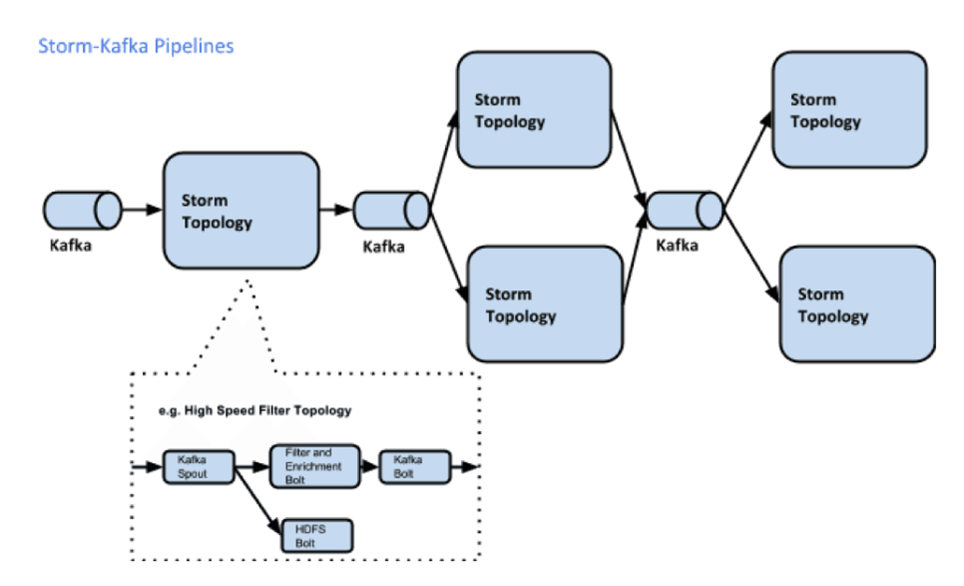
\includegraphics[scale=0.6]{image/storm-kafka-2.png}\\[0.5cm]
Figure 4. Apache Storm integration with Apache Kafka (2).
\end{center}
Here is Code\\
\begin{lstlisting}
	public class KafkaSpoutTopology
{
// ------------------------------ FIELDS ------------------------------

    private final static String KAFKA_HOST = "localhost:2181";
    private final static String NIMBUS_HOST = "192.168.1.152";
    private final static String KAFKA_TOPIC = "storm-test-topic";

    private final BrokerHosts brokerHosts;

// --------------------------- CONSTRUCTORS ---------------------------

    private KafkaSpoutTopology(String kafkaZookeeper)
    {
        brokerHosts = new ZkHosts(kafkaZookeeper);
    }

// --------------------------- main() method ---------------------------

    public static void main(String[] args) throws Exception
    {
        KafkaSpoutTopology kafkaSpoutTopology = new KafkaSpoutTopology(KAFKA_HOST);
        Config config = new Config();
//        config.put(Config.TOPOLOGY_TRIDENT_BATCH_EMIT_INTERVAL_MILLIS, 2000);
        config.put(Config.TOPOLOGY_MESSAGE_TIMEOUT_SECS, 30);

        StormTopology stormTopology = kafkaSpoutTopology.buildTopology();
        if (args != null && args.length > 0)
        {
            String name = args[0];
            config.put(Config.NIMBUS_HOST, NIMBUS_HOST); //YOUR NIMBUS'S IP
            config.put(Config.NIMBUS_THRIFT_PORT, 6627);    //int is expected here
            config.setNumWorkers(20);
            config.setMaxSpoutPending(5000);
            StormSubmitter.submitTopology(name, config, stormTopology);
        }
        else
        {
            config.setNumWorkers(2);
            config.setMaxTaskParallelism(Runtime.getRuntime().availableProcessors());
            LocalCluster cluster = new LocalCluster();
            cluster.submitTopology("kafka-storm-cassandra", config, stormTopology);
        }
    }

    private StormTopology buildTopology()
    {
        SpoutConfig kafkaConfig = new SpoutConfig(brokerHosts, KAFKA_TOPIC, "/tmp/kafka-logs", "storm-integration");
        kafkaConfig.scheme = new SchemeAsMultiScheme(new StringScheme());
//        kafkaConfig.startOffsetTime = System.currentTimeMillis();
        TopologyBuilder builder = new TopologyBuilder();
        builder.setSpout("words", new KafkaSpout(kafkaConfig), 10);
        builder.setBolt("write-to-cassandra", new CassandraWriterBolt()).shuffleGrouping("words");
//        builder.setBolt("notify", new NotifyBolt()).shuffleGrouping("write-to-cassandra");
//        builder.setBolt("write-to-elasticsearch", new ElasticSearchBolt()).shuffleGrouping("write-to-cassandra");
        return builder.createTopology();
    }
}
\end{lstlisting}

\begin{lstlisting}
class CassandraWriterBolt extends BaseRichBolt
{

    private static final Logger LOG = LoggerFactory.getLogger(CassandraWriterBolt.class);

    private final static String USERNAME = "vndev";
    private final static String PASSWORD = "123";
    private final static String HOST = "192.168.1.158";
    private final static String KEYSPACE = "dev";

    private Session session;
    private OutputCollector collector;

    @Override
    public void prepare(Map map, TopologyContext topologyContext, OutputCollector outputCollector)
    {
        this.collector = outputCollector;
    }

    @Override
    public void execute(Tuple tuple)
    {
        try
        {
            CassandraConnection connection = new CassandraConnection(HOST, KEYSPACE, USERNAME, PASSWORD);
            session = connection.getSession();
            LOG.info("content " + tuple.getString(0));
            boundCQLStatement(tuple, null);
            connection.close();
        }
        catch (Throwable t)
        {
            collector.reportError(t);
            collector.fail(tuple);
            LOG.error("tuple data error " + t.toString());
        }
    }

// --------------------- Interface IComponent ---------------------


    @Override
    public void declareOutputFields(OutputFieldsDeclarer declarer)
    {
        declarer.declare(new Fields("name", "post_id", "author_id", "content", "channel_ids", "published_time"));
    }

// -------------------------- OTHER METHODS --------------------------

    private void boundCQLStatement(Tuple input, UserActivity userActivity)
    {
        PreparedStatement statement = session.prepare(
                "INSERT INTO wordcounttable (source,word,count) VALUES (?, ?, ?);");
        BoundStatement boundStatement = new BoundStatement(statement);
        session.execute(boundStatement.bind(
                input.getString(0), "year", 1
        ));

    }
}
\end{lstlisting}
%%%%%%%%%%%%%%
\section{Kết Luận }\label{result}
\textbf{Kafka} có thể sử dụng làm "Spout" cho Apache Storm\\
\textbf{Apache Storm} có thể sử dụng các API của Trident (filter và function) để lọc và "emit" (phát ra) các Tuple mới cho Stream.\\
Một máy Storm cluster có thể có một hay nhiều Worker cho một hay nhiều topologies.  Mỗi tiến trình worker  thực thi executor cho riêng một topology.\\
 với một tiến trình worker, có thể có một hay nhiều executor có thể thực thi, với mỗi executor trở thành thread được sinh ra bởi worker process.
Mỗi executor có thể thực thi một hay nhiều tasks ó the same componemt(spout and bolt)\\
Mỗi task biểu thị quá trình xử lý dữ liệu thực tế...
%%%%%%%%%%%%%%
\section{Tài liệu Tham Khảo }
%%%%%%%%%%%%%%%%%%%%%%%%%%%%%%%%%
\begin{enumerate}
\item
\url{https://www.javaworld.com/article/3060078/big-data/big-data-messaging-with-kafka-part-1.html}
  \item \url{http://storm.apache.org}
\end{enumerate}

%%%%%%%%%%%%%%

\end{document}



